\documentclass[screen]{beamer}
\usepackage[T1]{fontenc}
\usepackage[latin1]{inputenc}
\usepackage{parskip}

% Bruk NTNU-temaet for beamer (her i bokmålvariant), alternativer er
% ntnunynorsk og ntnuenglish.
\usetheme{ntnuenglish}
 
% Angi tittelen, vi gir også en kortere variant som brukes nederst på
% hver slide:
\title[Paper 8]%
{Decomposable and Responsive Power Models}
\subtitle{for Multicore Processors using Performance Counters}

% Angir foredragsholder, også en (valgfri) kortversjon i
% hakeparanteser først som kommer nederst på hver slide:
\author[T. Runde and S. Hvatum]{Terje Runde and Stian Hvatum}

% Institusjon. Bruk gjerne disse slik det passer best med det du vil
% ha.  Valgfri kortversjon her også
\institute[NTNU]{Institutt for datateknikk og informatikk}

% Datoen blir også trykket på forsida. 
\date{28. october 2013}
%\date{} % Bruk denne hvis du ikke vil ha noe dato på forsida.

% Fra her av begynner selve dokumentet
\begin{document}

% Siden NTNU-malen har en annen bakgrunn på forsida, må dette gjøres
% i en egen kommando, ikke på vanlig beamer-måte:
\ntnutitlepage

% Her begynner første slide/frame, (nummer to etter forsida). 
\begin{frame}
    \frametitle{Motivation}

  \begin{itemize}
    \item Power wall
    \item A platform for online power-aware scheduling
  \end{itemize}

\end{frame}

\begin{frame}
    \frametitle{Observations}

    Current models\ldots

    \begin{itemize}
        \item \ldots are not fine-grained enough to model modern architectures
            \begin{itemize}
                \item Superscalarity
                \item Out-of-order execution
            \end{itemize}
        \item \ldots are only evaluated by their \emph{accuracy}
            \begin{itemize}
                \item We want \emph{responsiveness} too
            \end{itemize}
        \item \ldots does not apply to upcomming architectures
    \end{itemize}

    \pause

\textbf{Solution: Define power models}

\end{frame}

\begin{frame}
    \frametitle{Methodology}
    Prerequisite: An overview of the microarchitectural components
\end{frame}

\begin{frame}
    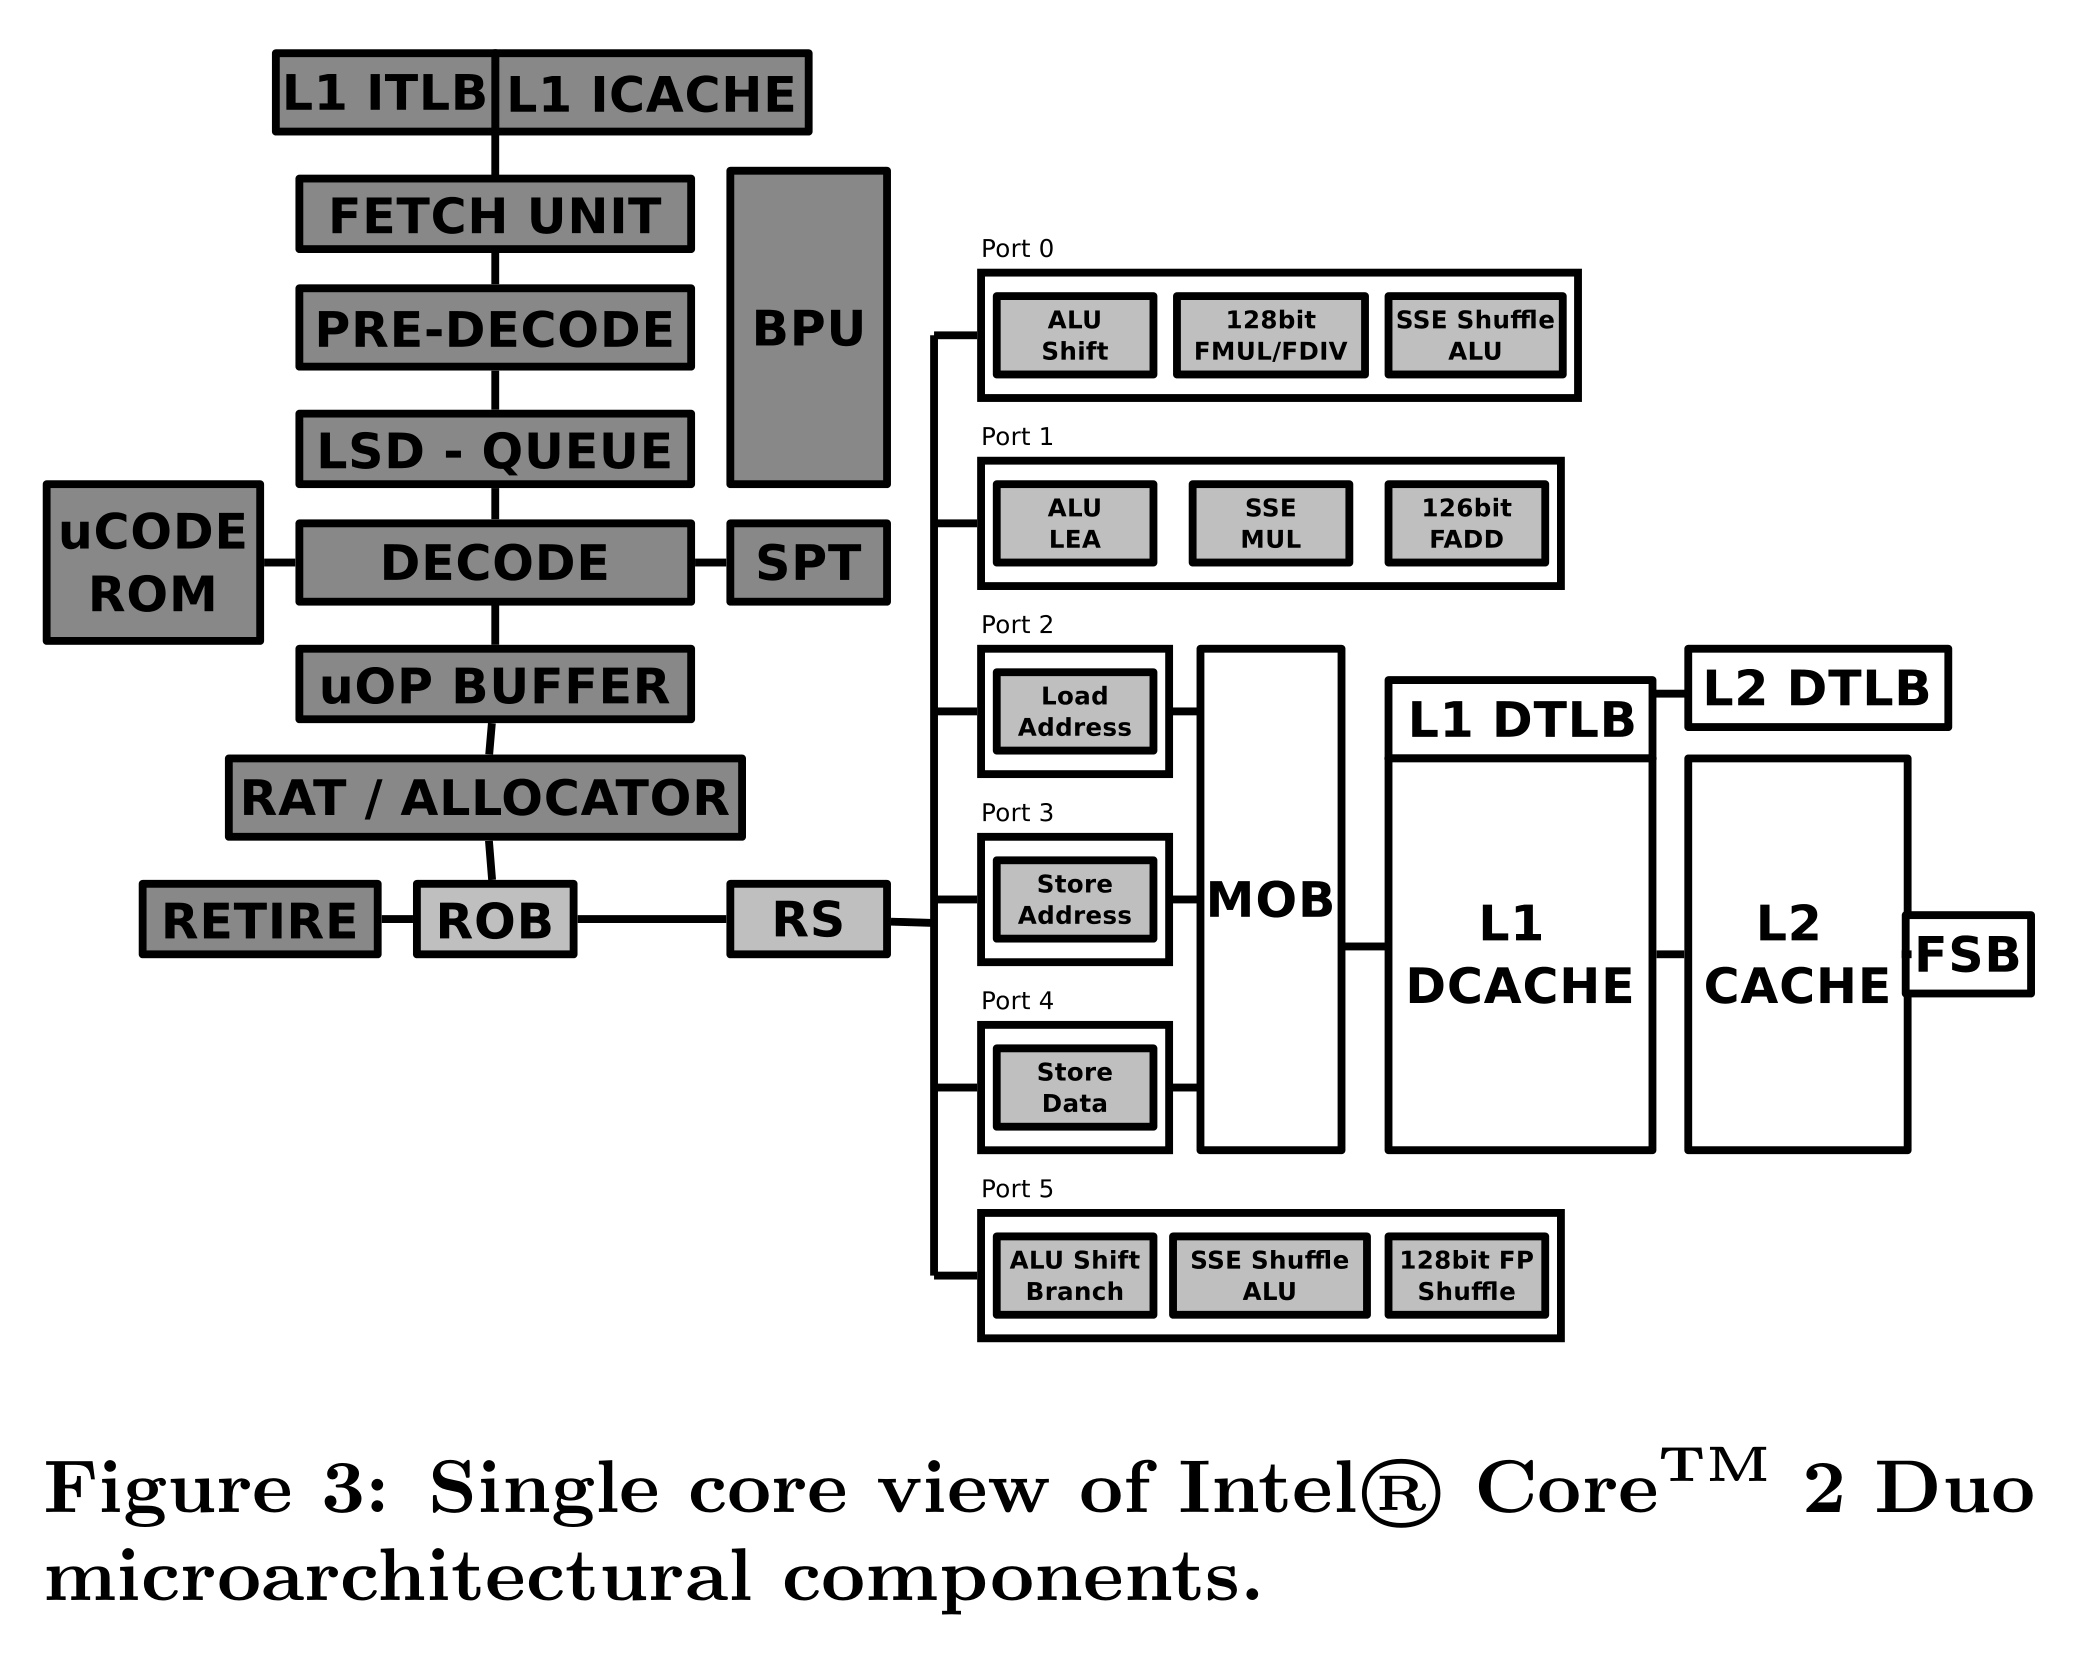
\includegraphics{Fig3}
\end{frame}

\begin{frame}
    \frametitle{Methodology}
    \textbf{Algorithm}
    \begin{figure}
    \begin{enumerate}
        \item Define power components
        \item Define training benchmarks
        \item Execute benchmarks and sample data
        \item Create model
    \end{enumerate}
    \end{figure}

\end{frame}



\begin{frame}
    \frametitle{Methodology}
    \textbf{Step 1: Defining the power components}

    \begin{itemize}
        \item Inspect the microarchitecture and isolate as much as possible
        \item Problem: Some components are shared
            \begin{itemize}
                \item Merge
            \end{itemize}
    \end{itemize}


\end{frame}

\begin{frame}
    \frametitle{Methodology}
    \textbf{Step 2: Define training benchmarks}

    \begin{itemize}
        \item Create micro-benchmarks to stress particular power components
        \item Use syntetic applications
        \item Decouple power components
        \item Intel Core 2 Duo specific: fxch instruction
    \end{itemize}


\end{frame}
\begin{frame}
    \frametitle{Methodology}
    \textbf{Step 3: Execute benchmarks and sample data}

    \begin{itemize}
        \item Run benchmarks created in the previous step
        \item Turn off as much as possible
    \end{itemize}
\end{frame}

\begin{frame}
    \frametitle{Methodology}
    \textbf{Step 4: Create model}

    \begin{itemize}
        \item Solve the linear system

            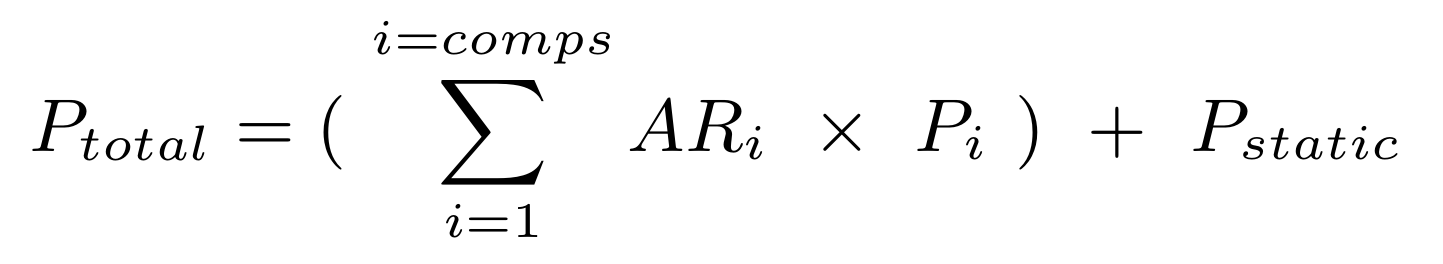
\includegraphics{Eq1}

        \item First solve the smallest subset where you are most confident with the results
    \end{itemize}

\end{frame}

\begin{frame}
    \frametitle{Validation - model correctness}

    \begin{itemize}
        \item All models performs about the same in terms of accuracy: \emph{Model accuracy has not improved}
        \item \ldots however, standard deviation decreases when tracking more components
    \end{itemize}

\end{frame}

\begin{frame}
    \frametitle{Validation - responsiveness}

    \begin{itemize}
        \item Phase detection algorithm
        \item {\ttfamily MICRO} are far more responsive

    \item Observation: 63\% of phases are (2,10] seconds long
        \begin{itemize}
            \item Long enough to overcome overhead of power aware policies
        \end{itemize}

    \end{itemize}

\end{frame}

\begin{frame}

    \frametitle{Conclusion}

   Responsiveness, decomposability and some accuracy is a power model must-have.

   It is hard to decompose proprietary architectures where details are under NDAs.

\end{frame}




    %  \begin{block}{Bokstittel}
    %    Comodo consequat.
    %  \end{block}
\end{document}
